\section{Gravitation \kuchling{140}}
Die Anziehung zwischen zwei Körpern heisst Gravitationskraft.

\begin{center}
	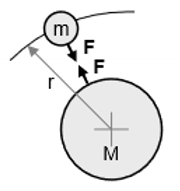
\includegraphics[height=8em]{./Images/gravitation.png}
\end{center}
\begin{formula}
	{F = G\frac{m_1m_2}{r^2}}
	F & Gravitationskraft & [N] \\
	m & Masse von Körper & [kg] \\
	G & Gravitationskonstante & [\frac{m^3}{kg \cdot s^2}] \\
	r & Abstand von Schwerpunkte & [m]
\end{formula}

\noindent\textbf{Konstanten}
\begin{align*}
	\text{Gravitationskonstante} &= 6.674 \cdot 10^{-11} \frac{m^3}{kg \cdot s^2} \\
	\text{Masse Erde} &= 5.974 \cdot 10^{24} kg \\
	\text{Radius Erde} &= 6.371 \cdot 10^{6} m
\end{align*}


\subsection{Fallbeschleunigung}
\begin{formula}
	{g = \frac{Gm}{r^2}}
	g & Fallbeschleunigung & [N] \\
	m & Masse von Körper & [kg] \\
	G & Gravitationskonstante & [\frac{m^3}{kg \cdot s^2}] \\
	r & Abstand von Schwerpunkte  & [m]
\end{formula}

\begin{center}
	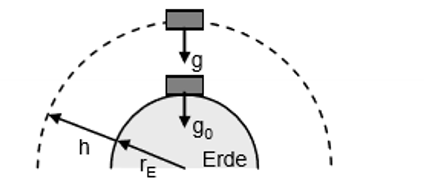
\includegraphics[height=8em]{./Images/fallbeschleunigung.png}
\end{center}
\begin{formula}
	{g = \frac{r_e^2 \cdot g_0}{(r_e + h)^2}}
	r_e & Radius Erde (o.ä.) & [kg] \\
	g_0 & Gravitation Erde & [\frac{m}{s^2}] \\
	h & Höhe über Radius Oberfläche. & [m]
\end{formula}

\subsection{Arbeit in Gravitation} \label{gravitationsarbeit}
\begin{center}
	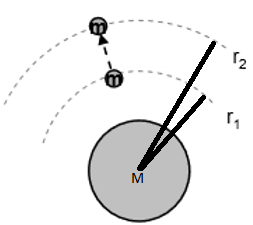
\includegraphics[height=8em]{./Images/gravitationspotental.png}
\end{center}
\begin{formula}
	{E_{Hub} = \\GMm\left(\frac{1}{r_1}-\frac{1}{r_2}\right)}
	M & Masse Erde (o.ä.) & [kg] \\
	m & Masse Körper & [kg] \\
	G & Gravitationskon. & [\frac{m^3}{kg \cdot s^2}] \\
	r & Abs. Schwerpunkt $m_1$ & [m]
\end{formula}


\begin{formula}
	{E_{Pot} = \frac{Gm_1m_2}{r}}
	m_1 & Masse Erde (o.ä.) & [kg] \\
	m_2 & Masse Körper & [kg] \\
	G & Gravitationskon. & [\frac{m^3}{kg \cdot s^2}] \\
	r & Abs. Schwerpunkt $m_1$ & [m]
\end{formula}

\subsection{Astronautische Geschwindigkeiten}
Mit der \textbf{Kreisbahngeschwindigkeit} $v_k$ kann ein Erdsatellit in beliebiger Höhe bestimmt werden.
\begin{formula}
	{v_k = \sqrt{\frac{GM}{r}}}
	
	v_k & Geschw. eines Objekts & [m/s] \\
	G & Gravitationskon. & [\frac{m^3}{kg \cdot s^2}] \\
	M & Masse Erde (o.ä.) & [kg] \\		
	r & Abs. Schwerpunkt $\leftrightarrow$ Objekt & [m]
\end{formula}

\begin{formula}
	{t = 2\pi r \cdot \frac{1}{\sqrt{\frac{GM}{r}}}}
	
	t & Umlaufzeit & [s]\\
	G & Gravitationskon. & [\frac{m^3}{kg \cdot s^2}] \\
	M & Masse Erde (o.ä.) & [kg] \\		
	r & Abs. Schwerpunkt $\leftrightarrow$ Objekt & [m] \\
\end{formula}

\noindent Mit der \textbf{Fluchtgeschwindigkeit} $v_f$ bestimmt die Mindestgeschwindigkeit, die ein Körper besitzen muss, um das Gravitationsfeld der Erde ohne Antrieb zu überwinden.

\begin{formula}
	{v_f &= \sqrt{\frac{2GM}{r}} \\ &= v_k\sqrt{2}}
	
	v_f & Geschw. eines Objekts & [m/s] \\
	G & Gravitationskon. & [\frac{m^3}{kg \cdot s^2}] \\
	M & Masse Erde (o.ä.) & [kg] \\		
	r & Abs. Schwerpunkt $\leftrightarrow$ Objekt & [m]
\end{formula}

\section{Rakete}
\begin{center}
	\includegraphics[width=0.5\columnwidth]{./Images/Rakete.png}
\end{center}

\begin{formula}
	{F_s &= u \cdot \frac{dm}{dt}}
\end{formula}

\begin{formula}
	{v(t) &= u \cdot \ln\left(\frac{m_0}{m_0 - \mu t}\right) - gt}
\end{formula}

\begin{formula}
	{h(t) &= \int_{0}^{x}v(t)dt}
\end{formula}

\begin{tabular}{>{$}l<{$} @{${}:{}$} l >{$}r<{$}}
	F_s & Schubkraft & [N] \\
	v & Fluggeschw. & [m/s] \\
	m_0 & Startmasse & [kg] \\	
	u & Strahlgeschw. rel. zur Rakete & [m/s] \\
	\mu & Verbrennungsgeschw. & [kg/s] \\
	h & Höhe & [m] \\
	x & Zeitpunkt & [s] \\
\end{tabular}


